\input{configuration}
\usepackage{soul}

\title{Lecture 28 --- Causal and Simulation Profiling }

\author{Patrick Lam \& Jeff Zarnett \\ \small \texttt{patrick.lam@uwaterloo.ca jzarnett@uwaterloo.ca}}
\institute{Department of Electrical and Computer Engineering \\
  University of Waterloo}
\date{\today}


\begin{document}

\begin{frame}
  \titlepage
 \end{frame}

\part{Causal Profiling}

\begin{frame}
	\partpage
\end{frame}

\begin{frame}
\frametitle{Causal Profiling}

If we have more than one slow thing, which do we want to optimize?

Scientific approach: do an experiment, see the impact, re-evaluate.

\begin{center}
	
\includegraphics[width=0.8\textwidth]{images/yeah_science.jpg}
\end{center}

\end{frame}


\begin{frame}
\frametitle{Causal Profiling}

Causal profiling lets us do what-if without code changes!

Example we'll discuss today: \alert{Coz}.


\end{frame}


\begin{frame}
\frametitle{Why Causal Profiling?}

Simple approach: look at the time and calculate what happens if \texttt{work()} runtime is reduced by 10\%.

This model is okay but it's not very realistic.

We actually want a simulation!


\end{frame}


\begin{frame}
\frametitle{Key Idea: Make Others Worse}

Key observation: speeding up one part is the same as slowing all others down.

How? Insert pauses.

Is that really equivalent to speeding up the target?

\end{frame}


\begin{frame}
\frametitle{Slowdown is Speedup}

\begin{center}
	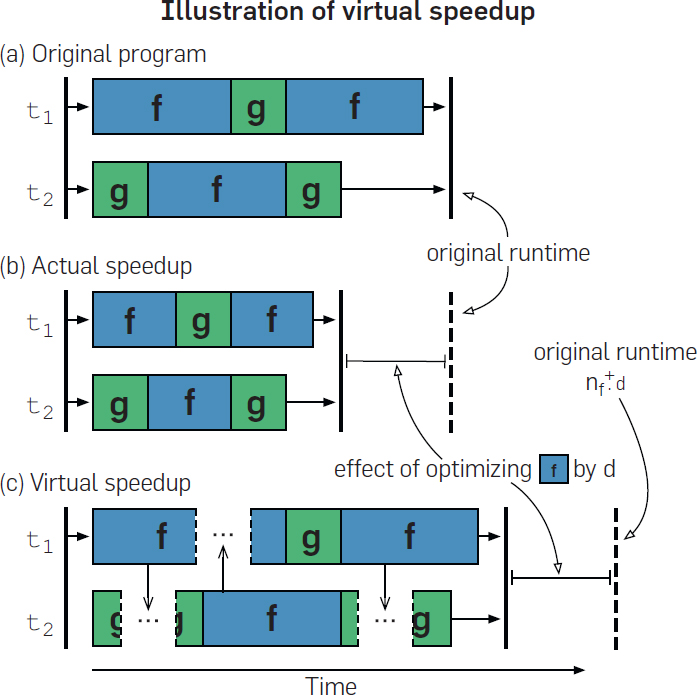
\includegraphics[width=0.6\textwidth]{images/virtual-speedup.jpg}
\end{center}

\end{frame}


\begin{frame}
\frametitle{Coz Graphs}

\begin{center}
	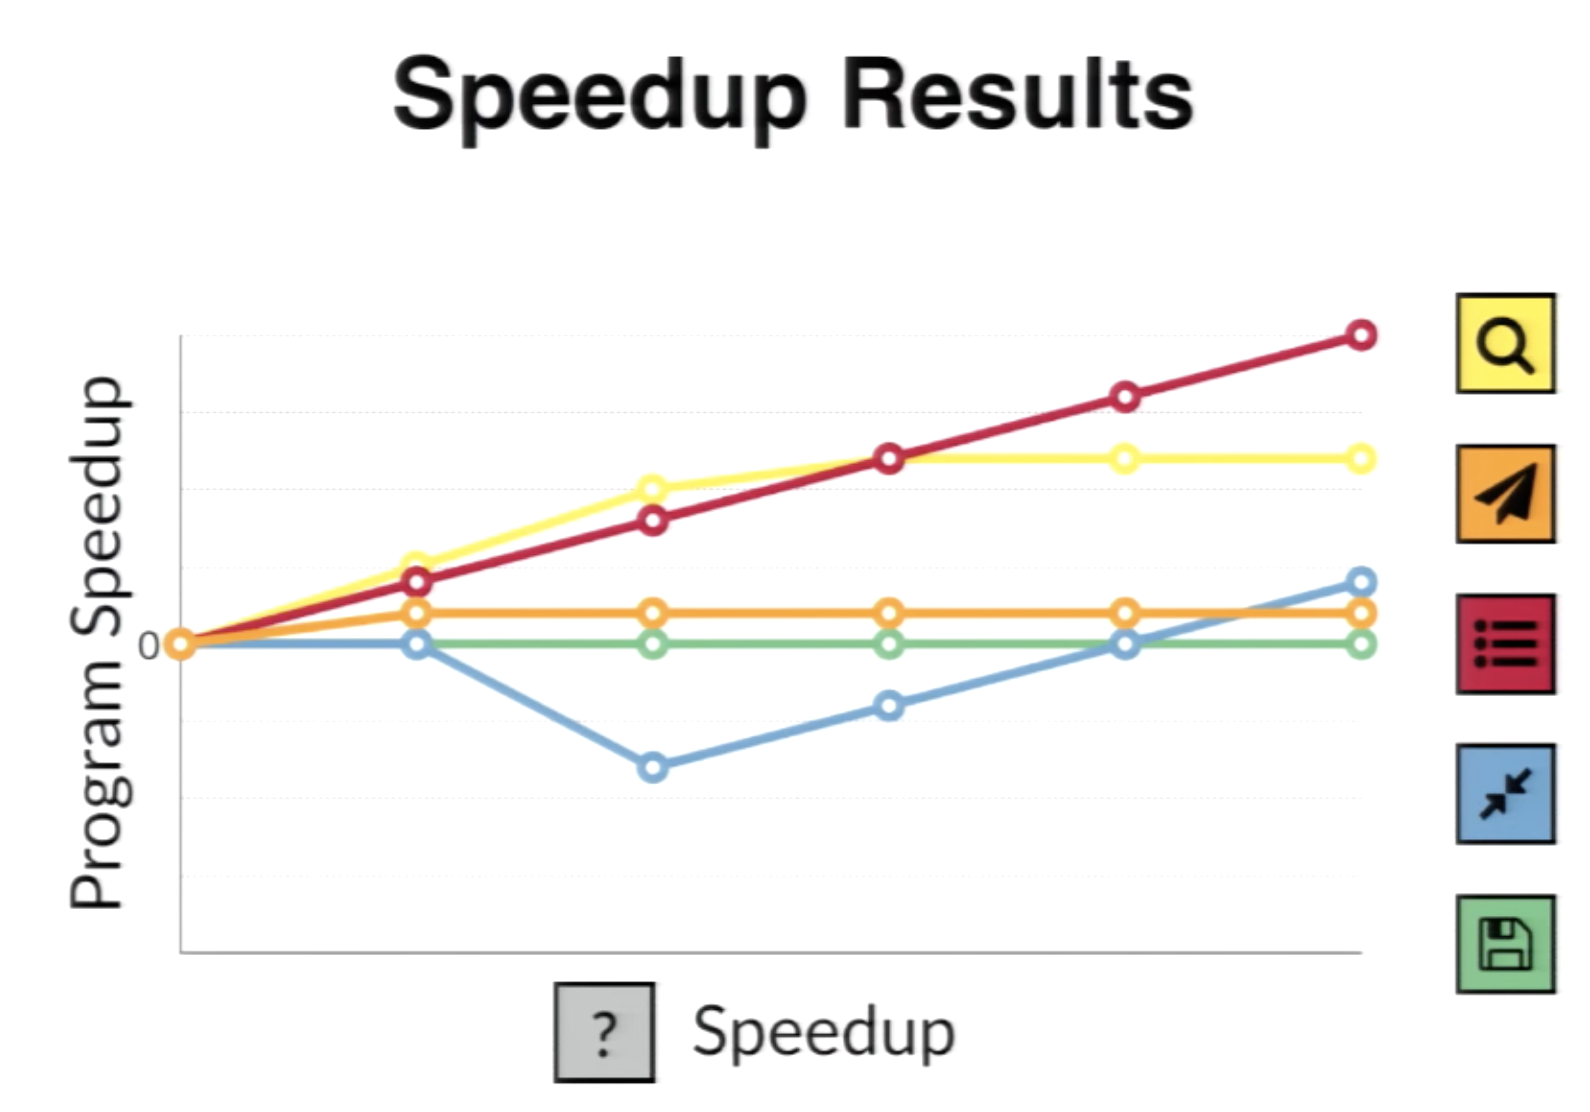
\includegraphics[width=\textwidth]{images/coz-speedup-graph.png}
\end{center}

\end{frame}


\begin{frame}
\frametitle{That Would Be Nice}
Just because hypothetically speeding up a particular part of the program would be beneficial, doesn't mean that it's possible to speed up that part.

We still need to assess what we can do and how difficult it would be.

\end{frame}


\begin{frame}
\frametitle{Does it Work?}

\begin{center}
	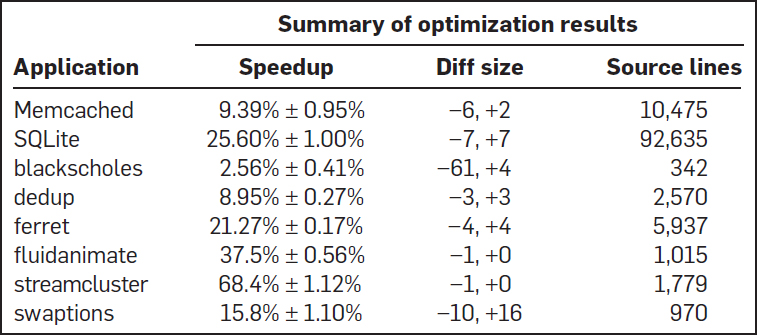
\includegraphics[width=\textwidth]{images/coz-speedup.jpg}
\end{center}

\end{frame}


\begin{frame}
\frametitle{Limitations, Overhead}

Only works on one machine where we have access to all threads.

Estimated overhead is 17.6\% total:\\
\quad 2.6\% startup debug information collection\\
\quad 4.8\% sampling\\
\quad 10.2\% inserted pauses

\end{frame}


\begin{frame}
\frametitle{More Details}

More details in the author presentation:

\url{https://www.youtube.com/watch?v=jE0V-p1odPg}

\end{frame}

\begin{frame}
\frametitle{Next Generation: \texttt{scoz}}
The next extension \texttt{scoz} is meant to address some shortcomings:

1. Inability to look at multi-process applications

2. Cases where the OS is the bottleneck.


(Reducing systems calls is a form of ``do less work'')

\end{frame}

\begin{frame}
\frametitle{The Goal: Core-Based System}

Instead of pausing threads, pause other cores.

(There are details about how to charge delays to the ``right'' core)

\begin{center}
	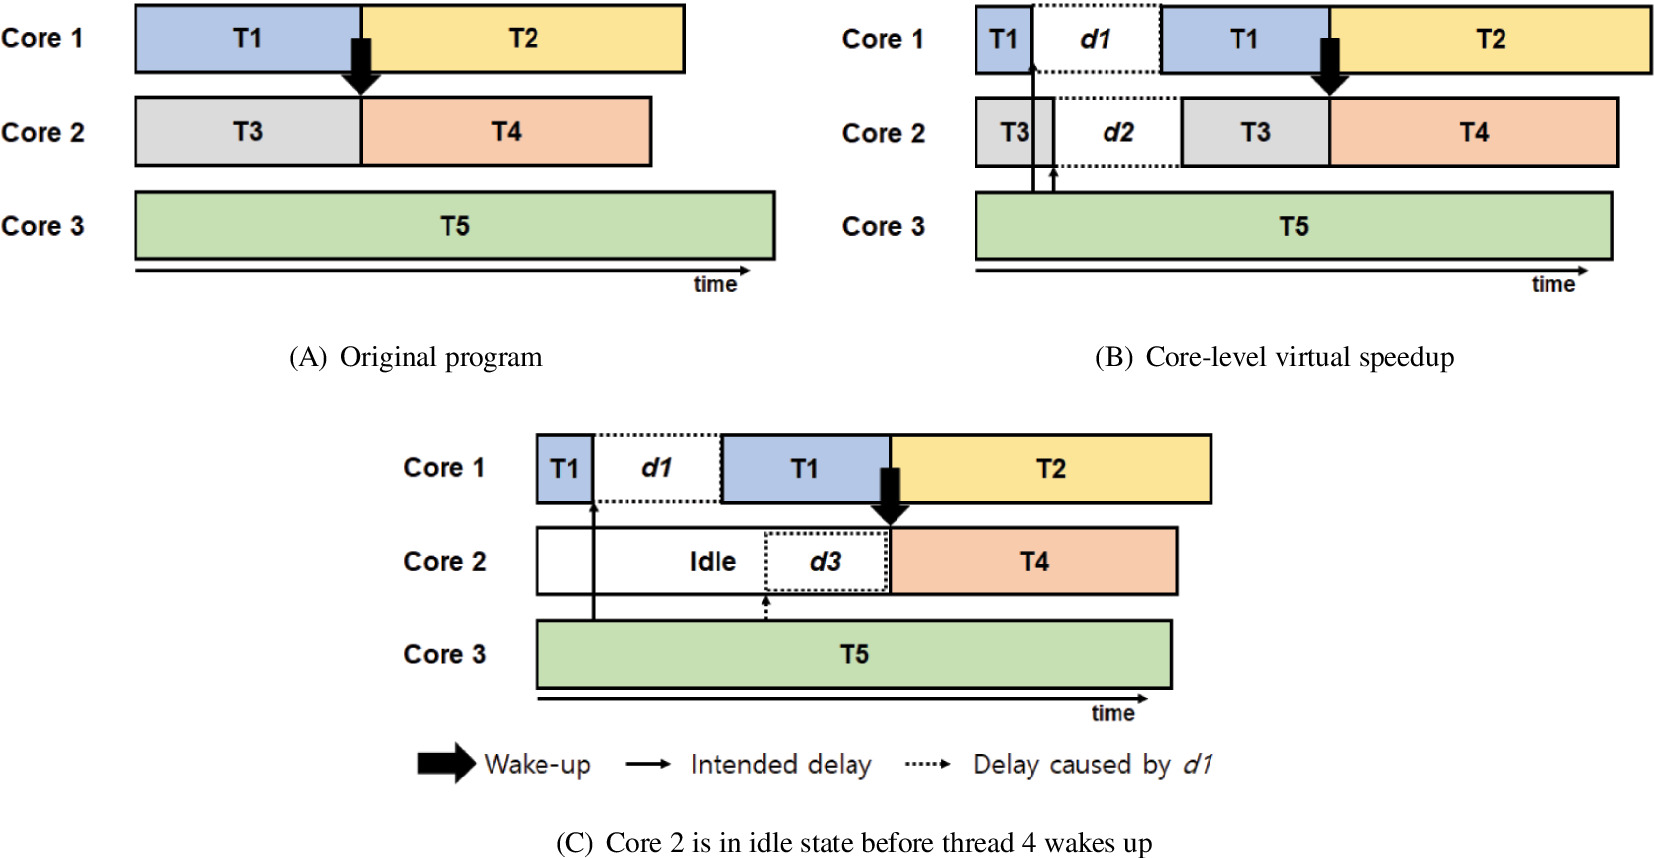
\includegraphics[width=0.8\textwidth]{images/scoz-delay.jpg}
\end{center}

\end{frame}

\begin{frame}
\frametitle{Implementation}

The implementation involves one profiler thread for each core to manage its behaviour. 

The thread is pinned to the core, and its purpose is primarily to call the \texttt{ndelay} interface (with preemption temporarily disabled) to stop execution.

\end{frame}

\part{Simulation Profiling}

\begin{frame}
	\partpage
\end{frame}

\begin{frame}
\frametitle{Simulations}

Causal profiling lets us use a simulation to decide what to do.

Let's apply this idea to some other things!

\end{frame}

\begin{frame}
\frametitle{Cachegrind}

This is much more performance oriented than the other two tools. 

 It runs simulation of how your program interacts with cache and evaluates how your program does on branch prediction.
 
 As we discussed earlier, cache misses and branch mispredicts have a huge impact on performance.
 
 Recall that a miss from the fastest cache results in a small penalty (10 cycles).
 
 A miss that requires going to memory requires about 200 cycles. 
 
 A mispredicted branch costs somewhere between 10-30 cycles.


\end{frame}

\begin{frame}
\frametitle{Cachegrind Reporting}

Cachegrind reports data about:
\begin{itemize}
	\item The First Level Instruction Cache (I1) [L1 Instruction Cache]
	\item The First Level Data Cache (D1) [L1 Data Cache]
	\item The Last Level Cache (LL) [L3 Cache].
\end{itemize}

Unlike normal Valgrind operation, you probably want to turn optimizations on.

\end{frame}

\begin{frame}[fragile]
\frametitle{Sim-u-laaaaate!}
{\scriptsize

\begin{verbatim}
jz@Loki:~/ece254$ valgrind --tool=cachegrind --branch-sim=yes ./search

--16559-- warning: L3 cache found, using its data for the LL simulation.
Found at 11 by thread 1 
Found at 22 by thread 3 
==16559== 
==16559== I   refs:      310,670
==16559== I1  misses:      1,700
==16559== LLi misses:      1,292
==16559== I1  miss rate:    0.54%
==16559== LLi miss rate:    0.41%
==16559== 
==16559== D   refs:      114,078  (77,789 rd   + 36,289 wr)
==16559== D1  misses:      4,398  ( 3,360 rd   +  1,038 wr)
==16559== LLd misses:      3,252  ( 2,337 rd   +    915 wr)
==16559== D1  miss rate:     3.8% (   4.3%     +    2.8%  )
==16559== LLd miss rate:     2.8% (   3.0%     +    2.5%  )
==16559== 
==16559== LL refs:         6,098  ( 5,060 rd   +  1,038 wr)
==16559== LL misses:       4,544  ( 3,629 rd   +    915 wr)
==16559== LL miss rate:      1.0% (   0.9%     +    2.5%  )
==16559== 
==16559== Branches:       66,622  (65,097 cond +  1,525 ind)
==16559== Mispredicts:     7,202  ( 6,699 cond +    503 ind)
==16559== Mispred rate:     10.8% (  10.2%     +   32.9%   )

\end{verbatim}
}

\end{frame}

\begin{frame}[fragile]
\frametitle{Optimizations: Enabled!}
{\scriptsize
\begin{verbatim}
jz@Loki:~/ece254$ valgrind --tool=cachegrind --branch-sim=yes ./search

--16618-- warning: L3 cache found, using its data for the LL simulation.
Found at 11 by thread 1 
Found at 22 by thread 3 
==16618== 
==16618== I   refs:      306,169
==16618== I1  misses:      1,652
==16618== LLi misses:      1,286
==16618== I1  miss rate:    0.53%
==16618== LLi miss rate:    0.42%
==16618== 
==16618== D   refs:      112,015  (76,522 rd   + 35,493 wr)
==16618== D1  misses:      4,328  ( 3,353 rd   +    975 wr)
==16618== LLd misses:      3,201  ( 2,337 rd   +    864 wr)
==16618== D1  miss rate:     3.8% (   4.3%     +    2.7%  )
==16618== LLd miss rate:     2.8% (   3.0%     +    2.4%  )
==16618== 
==16618== LL refs:         5,980  ( 5,005 rd   +    975 wr)
==16618== LL misses:       4,487  ( 3,623 rd   +    864 wr)
==16618== LL miss rate:      1.0% (   0.9%     +    2.4%  )
==16618== 
==16618== Branches:       65,827  (64,352 cond +  1,475 ind)
==16618== Mispredicts:     7,109  ( 6,596 cond +    513 ind)
==16618== Mispred rate:     10.7% (  10.2%     +   34.7%   )
\end{verbatim}
}

\end{frame}

\begin{frame}
\frametitle{Results Analysis}


Interesting results: our data and instruction miss rates went down marginally but the branch mispredict rates went up!

Well sort of - there were fewer branches and thus fewer we got wrong as well as fewer we got right. 

So the total cycles lost to mispredicts went down. 

Is this an overall win for the code? Yes. 


\end{frame}
\begin{frame}
\frametitle{Do the Math}

In some cases it's not so clear cut, and we could do a small calculation. 

If we just take a look at the LL misses (4~544 vs 4~487) and assume they take 200 cycles, and the branch miss penalty is 200 cycles, it went from 908~800 wasted cycles to 897~400; a decrease of 11~400 cycles.

  Repeat for each of the measures and sum them up to determine if things got better overall and by how much.

\end{frame}
\begin{frame}
\frametitle{Cachegrind Detailed Output}

Cachegrind also produces a more detailed output file, titled cachegrind.out.<pid> (the PID in the example is 16618). 

This file is not especially human-readable, but we can ask the associated tool \texttt{cg\_annotate} to break it down for us.

The output is way too big for slides.

\end{frame}
\begin{frame}
\frametitle{Advanced Cachegrind}

Cachegrind is very... verbose... and it can be very hard to come up with useful changes based on what you see... 

Assuming your eyes don't glaze over when you see the numbers. 

Probably the biggest performance impact is last level cache misses (those appear as DLmr or DLmw). 

You might also try to look at the Bcm and Bim (branch mispredictions) to see if you can give some better hints. 
\end{frame}
\begin{frame}
\frametitle{Really Advanced Cachegrind}

This is a good way to validate that your changes actually worked!

Showing your manager (executive) WHY a change worked is more convincing...

\end{frame}

\begin{frame}
\frametitle{Simulations as Perf Debugging}

\begin{center}
	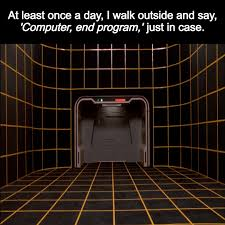
\includegraphics[width=0.4\textwidth]{images/endprogram.jpg}
\end{center}

Executing in a simulation allows for more than just counting the number of cache misses or a pipeline stalls -- you can see how we got there.

\end{frame}

\begin{frame}
\frametitle{Simulation Example}

Docs for TMS320C55x Digital Signal Processing platform by Texas Instruments.

Get more exact values of counts, cache misses, CPU stalls...\\
\quad And you can halt on events to look into them!

\end{frame}

\begin{frame}
\frametitle{Miri}

\begin{center}
	
\includegraphics[width=0.7\textwidth]{images/miri.jpg}
\end{center}

Everyone was extremely cool about the duplicate Earth...

\end{frame}

\begin{frame}
\frametitle{Miri \& Valgrind}

Miri has a lot of similarities with Valgrind!

I think its real intended use is to detect issues in \texttt{unsafe} code.\\
\quad Array bounds violations, reading uninitialized memory, memory leaks...

\begin{center}
	
\includegraphics[width=0.3\textwidth]{images/dothathere.jpg}
\end{center}

... Well. Except for launching GPU code.

\end{frame}

\begin{frame}[fragile]
\frametitle{Let's Do an Example}

To run, use the miri option and it will generate a \texttt{crox} directory with some file in it; process that file with the \texttt{crox} tool to generate a json file that can be read in chrome dev tools:

\begin{lstlisting}
MIRIFLAGS="-Zmiri-disable-isolation -Zmiri-measureme=crox" cargo +nightly miri run
\end{lstlisting}

It produces a flamegraph-style graph!

\end{frame}

\begin{frame}
\frametitle{Miri Example}

\begin{center}
	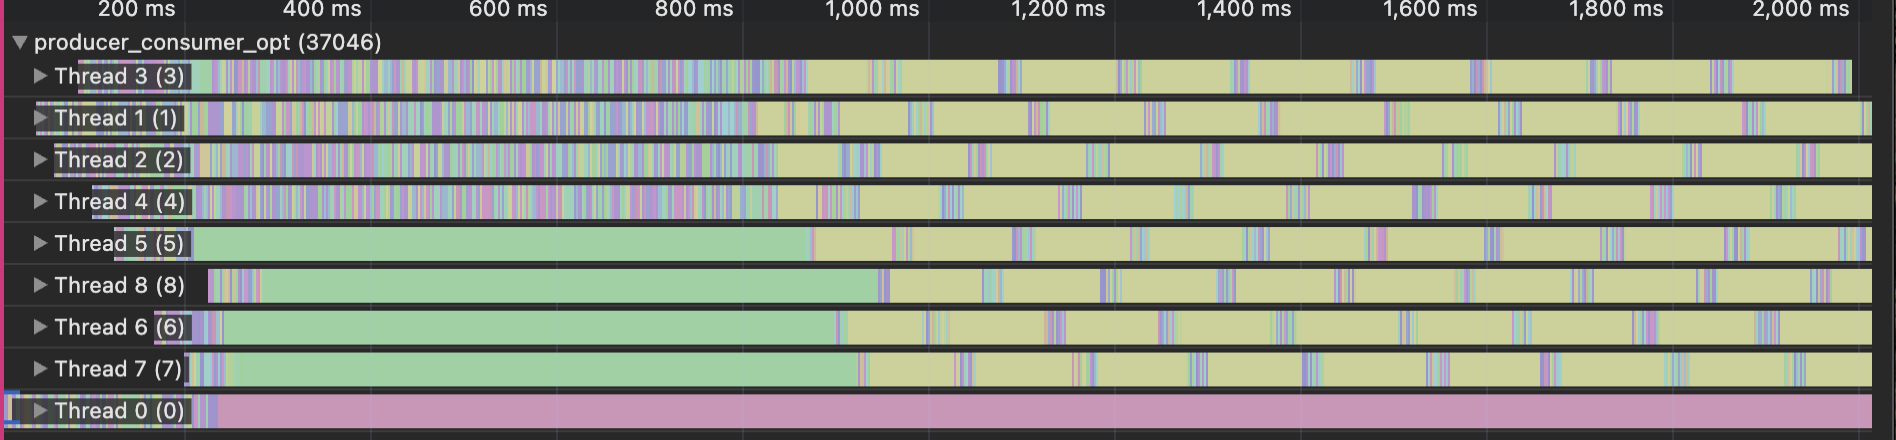
\includegraphics[width=\textwidth]{images/miri-pco1.png}
\end{center}

\end{frame}

\begin{frame}
\frametitle{Miri Example}

\begin{center}
	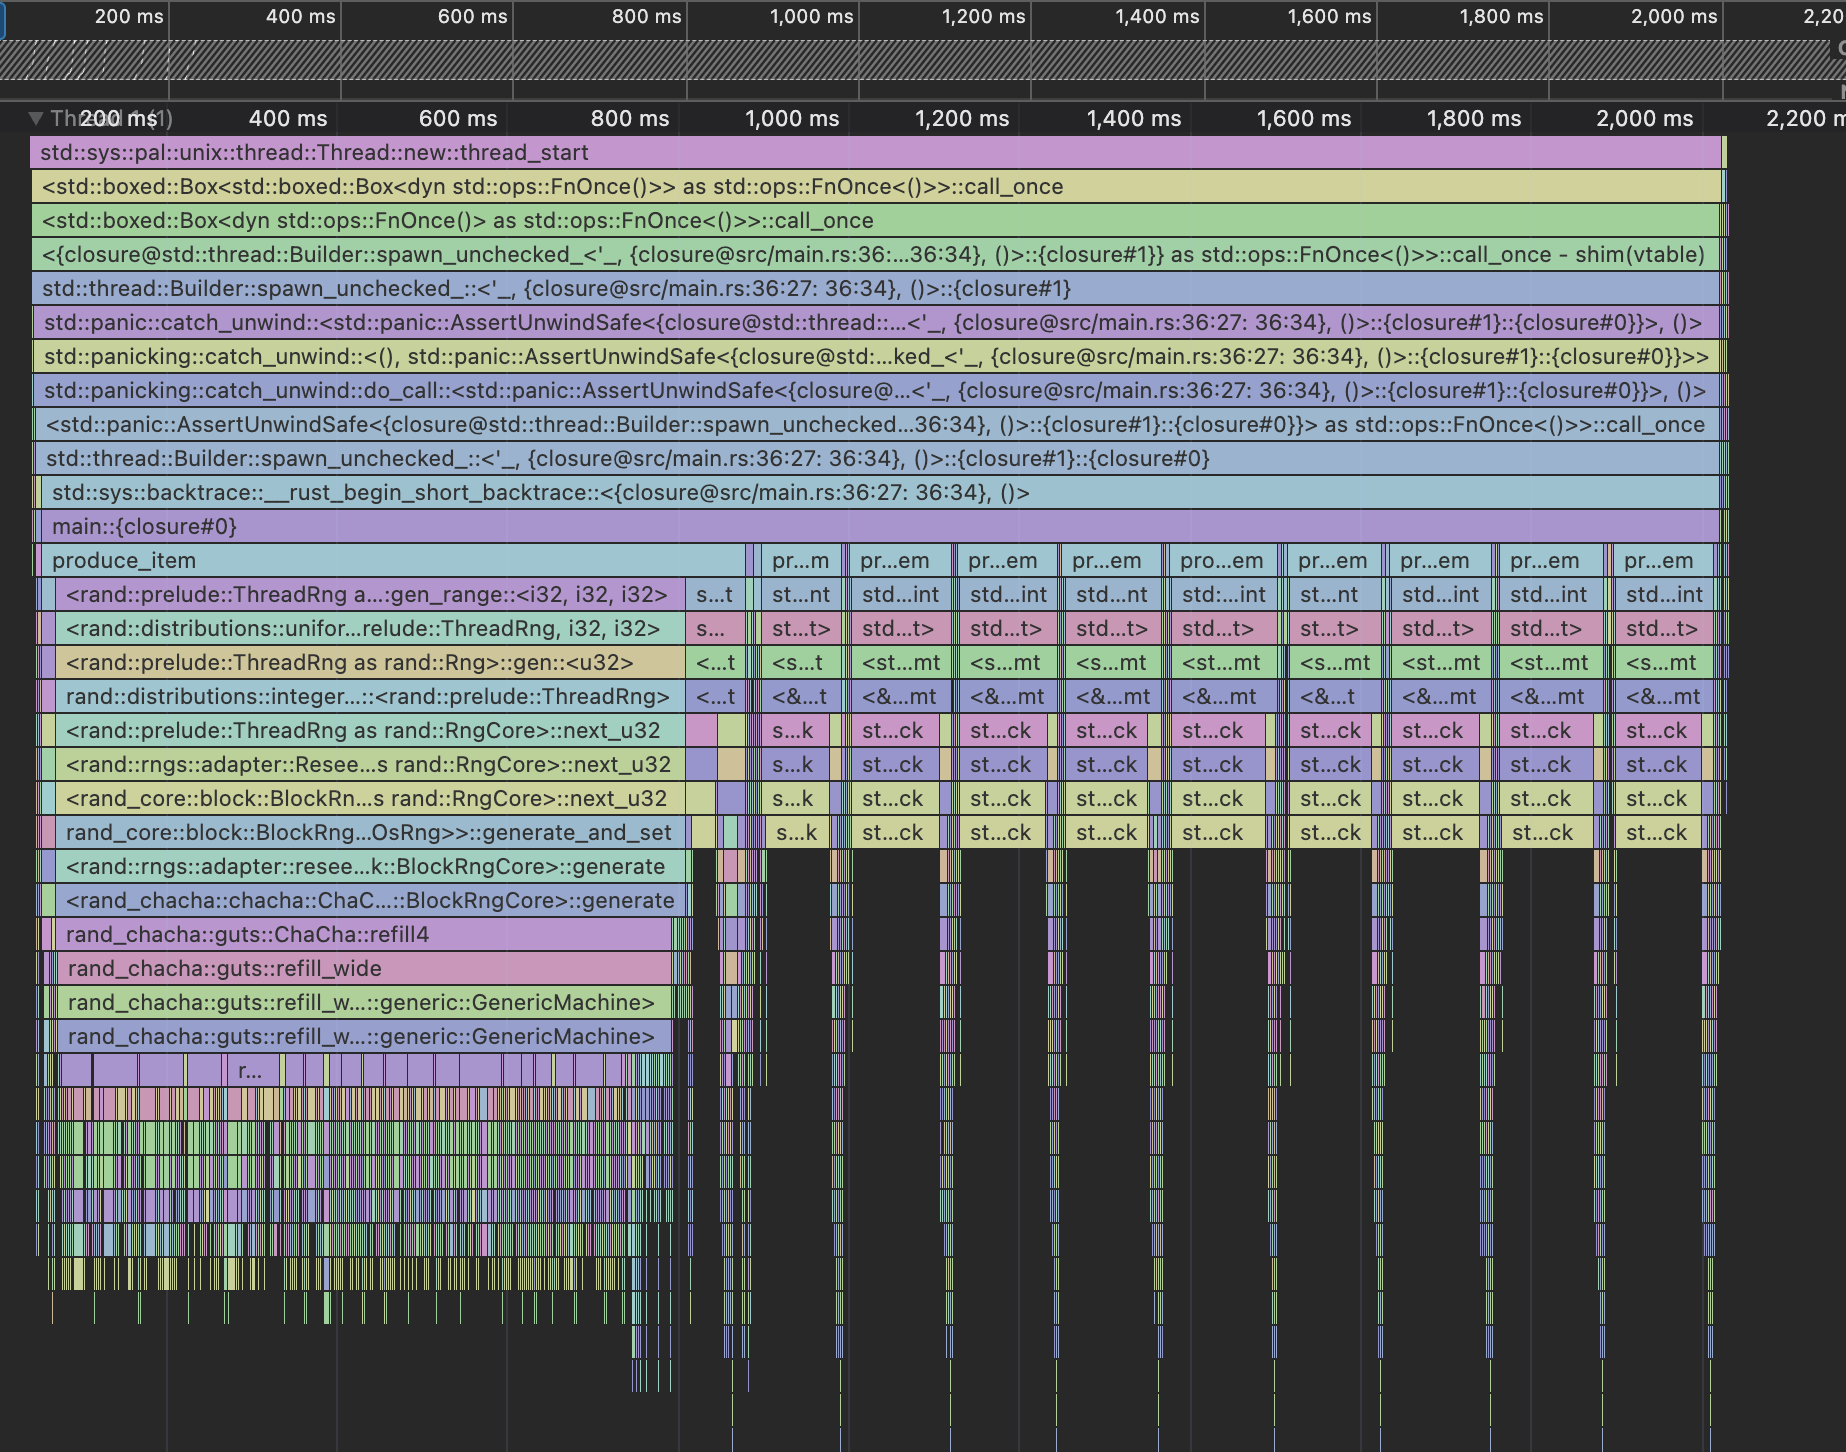
\includegraphics[width=0.85\textwidth]{images/miri-pco2.png}
\end{center}

\end{frame}

\begin{frame}
\frametitle{Miri Drawbacks}

Like Valgrind, it makes the program run much, much slower.

The article got a lot of comments about improving the debug version rather than the release one.

That is true, but it's meant to be used in the change-run-evaluate loop!

\end{frame}

\end{document}


